\documentclass[a4paper ]{article}
\usepackage{graphicx}
\usepackage[letterpaper, landscape, margin=2in]{geometry}
\geometry{
	paper=a4paper, % Change to letterpaper for US letter
	inner=0.5cm, % Inner margin
	outer=0.5cm, % Outer margin
	bindingoffset=0.01cm, % Binding offset
	top=0.5cm, % Top margin
	bottom=0.5cm, % Bottom margin
	%showframe, % Uncomment to show how the type block is set on the page
}
\usepackage[utf8]{inputenc}
%\usepackage{natbib}

\begin{document}
- - -

\vspace{50mm}
\begin{center}
{\Huge \textsc{\textbf{Savage Dickey}}}\\
{\Huge \textsc{\textbf{Comparing Prior and Posterior densities at the 'no differences' point}}}\\
\vspace{20mm}
\end{center}

\begin{center}
\textit{\huge Are the prior and posterior actually comparable?}\\
\bigskip
\end{center}

\begin{center}
\textit{\huge Adriana F. Chávez De la Peña}\\
\end{center}

\begin{center}
\vfill
\textit{\huge adrifelcha@gmail.com}\\
\end{center}

\newpage



---
\begin{center}
{\LARGE \textbf{(Reminder)} }\\
{\small \textsc{The model looked like:}}\\
\end{center}
\begin{figure}[h]
\centering
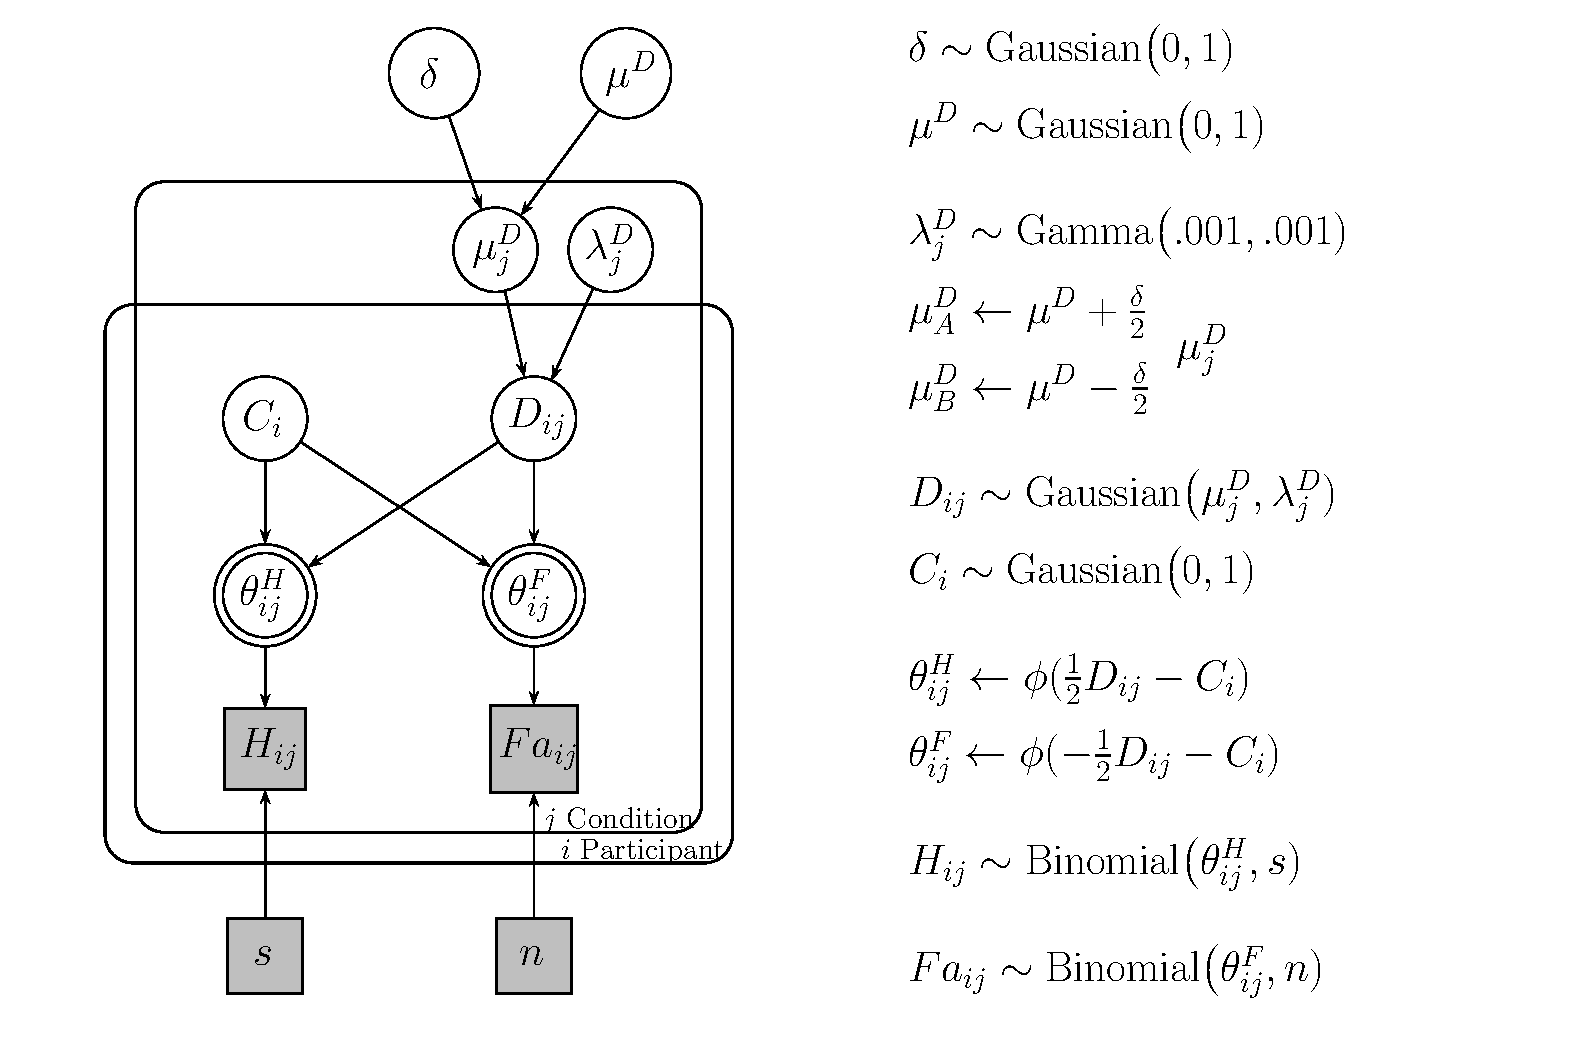
\includegraphics[width=.8\textwidth]{Figures/Delta_Michael}
\end{figure}
\clearpage


---
I plotted the density of the posterior along with the density of a prior (norm(0,1)) which is specifically composed by the same amount of samples that our model extracts for the posterior $prior <- rnorm((number of iterations-number of burnins), mean 0, sd =1)$, and then I estimated the ratio of their densities at $0$.
\begin{figure}[h]
\centering
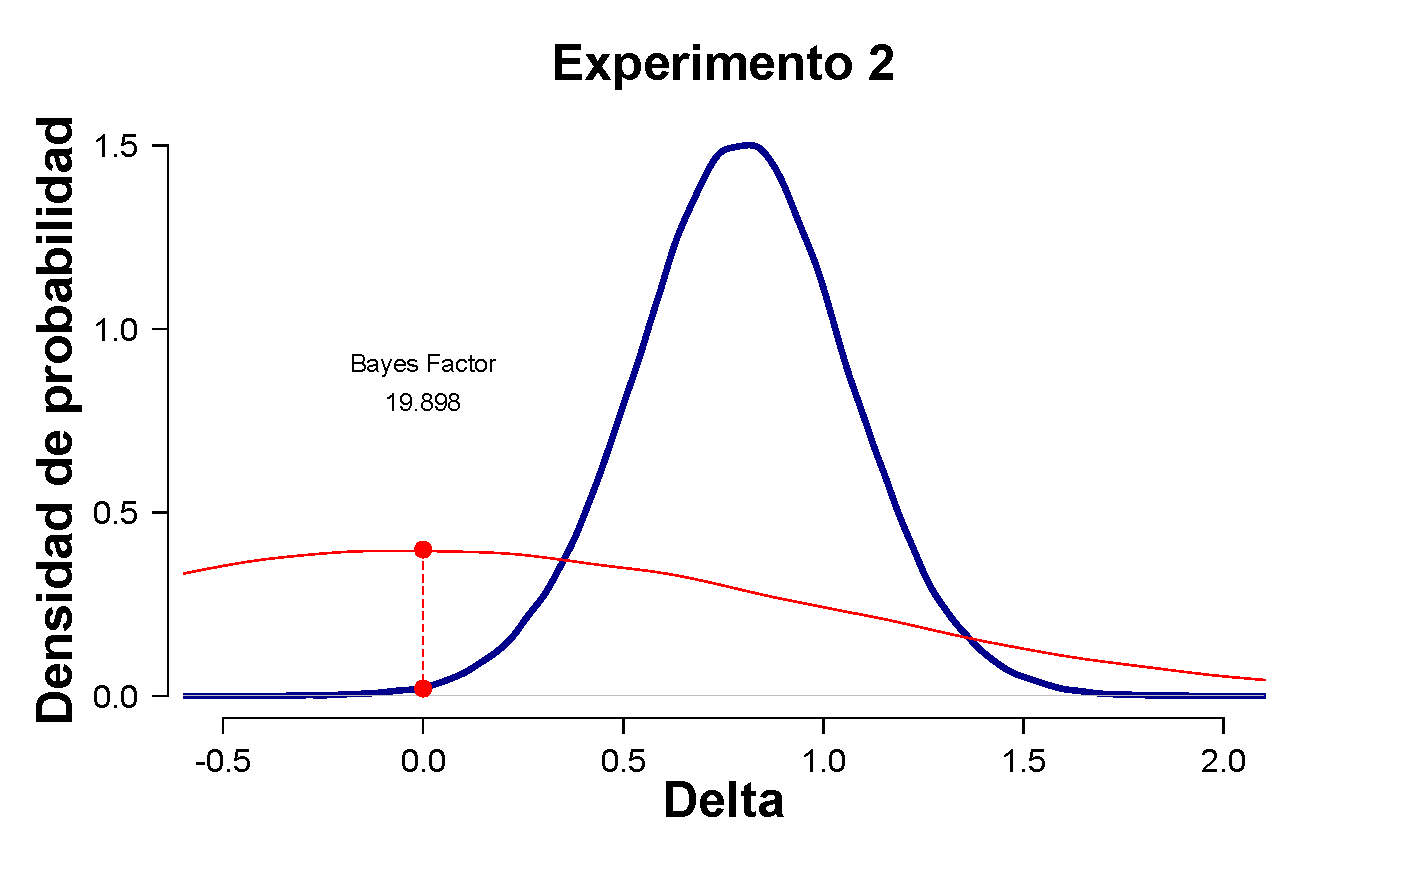
\includegraphics[width=.5\textwidth]{Figures/Delta_SavageDickey}
\end{figure}

However, it still looks like the prior is unusually shorter than the posterior.
\clearpage


---
I plotted the individual histograms for each distribution (prior and posterior) to see how their densities looked like. The results were consistent with the previous graphs: posterior seems to accumulate higher values of densities than the prior, but also the range of values covered on their x axis is quite different (the prior being a normal which goes from -4 to 4; the posterior only covers from -0.5 to 2).

\begin{figure}[h]
\centering
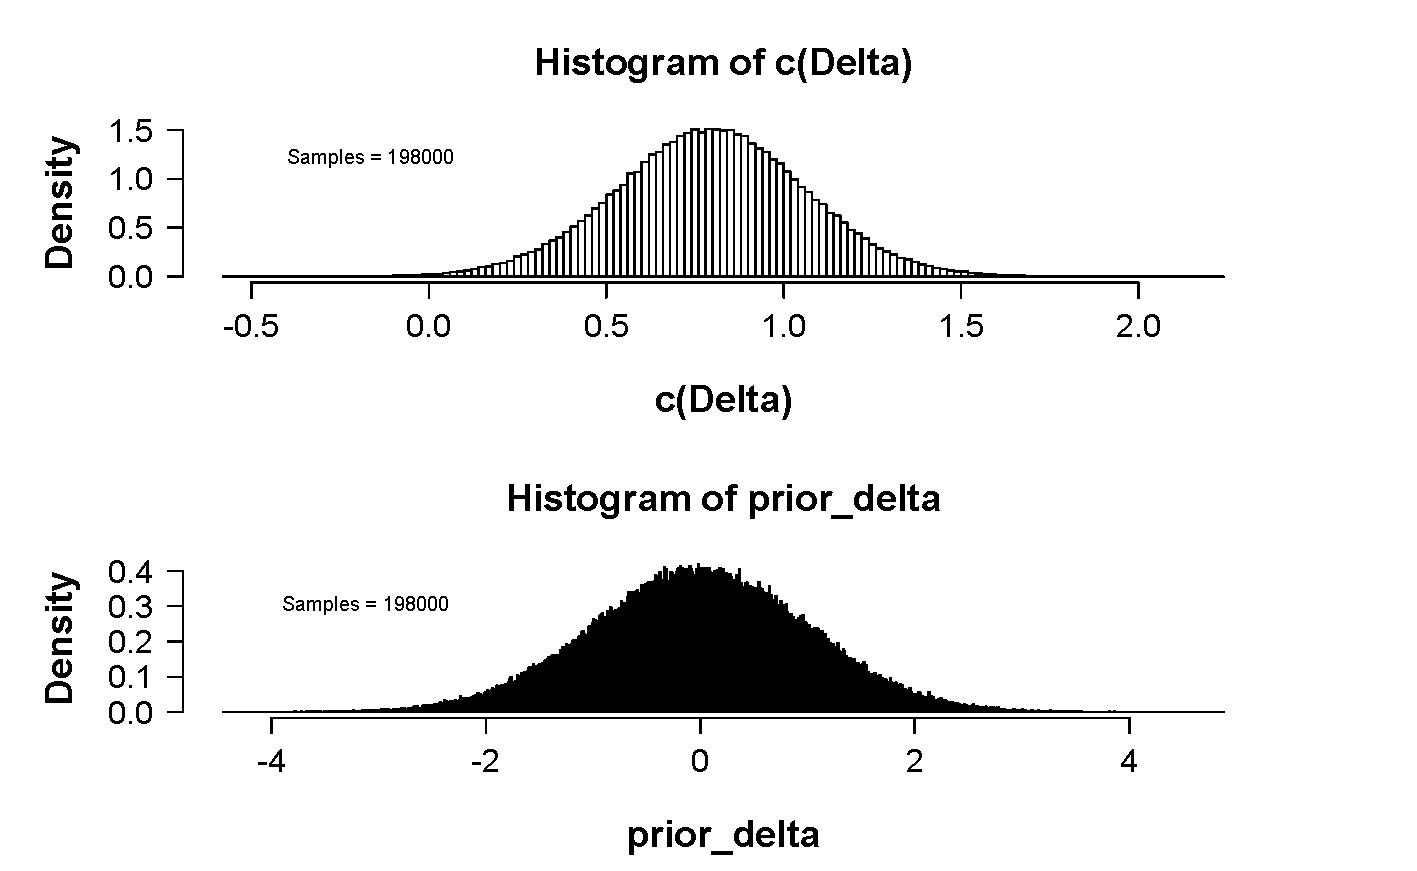
\includegraphics[width=.8\textwidth]{Figures/Delta_PriorPosteriorHist}
\end{figure}
\clearpage


I think that I'm doing the Savage Dickey thing right, even thought the heights of each distribution seem to be different.\\

I just wanted to make sure that my orthodox method for making the prior and posterior distributions "homogeneous" made sense (by just adjusting the amount of samples contained in the prior distribution to be equal to the samples extracted by the model for the posterior.)
 



\end{document}